\documentclass[a4paper,10pt]{article}
%\documentclass[a4paper,10pt]{scrartcl}

\usepackage[utf8x]{inputenc}
\usepackage{amsmath}
\usepackage{graphicx}
\usepackage{cancel} 

\title{HW\pound3-P1}
\author{Christopher Stricklan}
\date{02/13/2011}

\pdfinfo{%
  /Title    (HW#3-P1)
  /Author   (Christopher Stricklan)
  /Creator  (Christopher Stricklan)
  /Producer (Christopher Stricklan)
  /Subject  (EE5390-FDTD)
  /Keywords (FDTD)
}

\begin{document}
%\maketitle
\textbf{Maxwell's Equations}

\begin{equation}
  \nabla \cdot \vec{D}(t)=\rho_{v}(t)
\end{equation}

\begin{equation}
  \nabla \cdot \vec{B}(t)=0
\end{equation}

\begin{equation}
  \nabla \times \vec{E}(t) = -\frac{\partial \vec{B}(t)}{\partial t}
\end{equation}

\begin{equation}
  \nabla \times \vec{H}(t) = \vec{J} + \frac{\partial\vec{D}(t)}{\partial t}
\end{equation}
                                                                                   

\textbf{Constitutive relations}
\begin{equation}
  \label{eq:constitutive1}
  \vec{D} = [\epsilon(t)]*\vec{E}(t)
\end{equation}

\begin{equation}
  \label{eq:constitutive2}
  \vec{B} = [\mu(t)]*\vec{H}(t)
\end{equation}


\textbf{Eliminate Divergence}

Our use of the Yee Grid Scheme alows us to elimate divergence via equations \eqref{eq:Divergence1} and \eqref{eq:Divergence2}

\begin{equation} 
  \label{eq:Divergence1}
  \nabla \cdot (\epsilon\vec{E}) = 0
\end{equation}

\begin{equation} 
  \label{eq:Divergence2}
  \nabla \cdot(\mu\vec{H}) = 0
\end{equation}

This also allows for the centering of the fields invoked by the curl equations Figure \ref{fig:YeeGridWithCurls}

\begin{figure}[h]
  \centering
    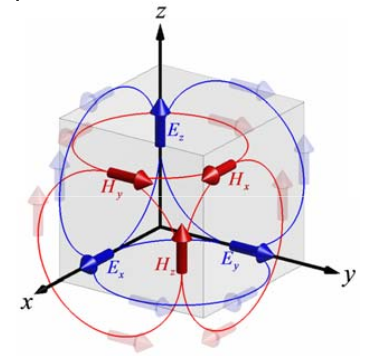
\includegraphics[width=0.5\textwidth]{YeeGrid.png}
  \caption{Yee Grid}
  \label{fig:YeeGridWithCurls}
\end{figure}
	
\textbf{Substitution}

Because we have satisfied the divergence equations by using the Yee Grid Scheme, we are now able to focus on the curl equations with our constituive relation equations \eqref{eq:constitutive1} and \eqref{eq:constitutive2} subsituted in.  We are also not injecting a Source.

\begin{equation*}
 \mbox{Where }\vec{J} = 0
\end{equation*}


\begin{equation}
  \nabla \times \vec{E}(t) = -[\mu]\frac{\partial \vec{H}(t)}{\partial t}
\end{equation}


\begin{equation}
   \nabla \times \vec{H}(t) = [\epsilon]\frac{\partial\vec{H}(t)}{\partial t}
\end{equation}


\textbf{Normalize Magnetic Field}

The Electric and Magnetic Fields are three orders of magnitude different.  Rounding errors can propagate through our simulation, therefore we require that we normalize a Field.  In this case we are normalizing the Magnetic Field.

\begin{align}
  \vec{\tilde{H}} = \sqrt{\frac{\mu_0}{\epsilon_0}}\vec{H}
  \Longrightarrow 
  \nabla \times \vec{E} = -\frac{[\mu_r]}{c_0}\frac{\partial \vec{\tilde{H}}}{\partial t}\\
  \nabla \times \vec{\tilde{H}} =  \frac{[\epsilon_r]}{c_0}\frac{\partial \vec{E}}{\partial t}\notag
\end{align}


\textbf{Expand Curl Equations}

\begin{align}
  \nabla \times \vec{E} = -\frac{[\mu_r]}{c_0}\frac{\partial \vec{\tilde{H}}}{\partial t}
  \Longrightarrow\\
  \frac{\partial E_z}{\partial y} - \frac{\partial E_y}{\partial z} = -\frac{1}{c_0}\left(\mu_{xx} \frac{\partial\tilde{H}_x}{\partial t} + \mu_{xy} \frac{\partial\tilde{H}_y}{\partial t} + \mu_{xz} \frac{\partial\tilde{H}_z}{\partial t}\right)\notag\\
  \frac{\partial E_x}{\partial z} - \frac{\partial E_z}{\partial x} = -\frac{1}{c_0}\left(\mu_{yx} \frac{\partial\tilde{H}_x}{\partial t} + \mu_{yy} \frac{\partial\tilde{H}_y}{\partial t} + \mu_{yz} \frac{\partial\tilde{H}_z}{\partial t}\right)\notag\\
  \frac{\partial E_y}{\partial x} - \frac{\partial E_x}{\partial y} = -\frac{1}{c_0}\left(\mu_{zx} \frac{\partial\tilde{H}_x}{\partial t} + \mu_{zy} \frac{\partial\tilde{H}_y}{\partial t} + \mu_{zz} \frac{\partial\tilde{H}_z}{\partial t}\right)\notag
\end{align}

\begin{align}
  \nabla \times \vec{\tilde{H}} =  \frac{[\epsilon_r]}{c_0}\frac{\partial \vec{E}}{\partial t}
  \Longrightarrow\\
  \frac{\partial \tilde{H}_z}{\partial y} - \frac{\partial \tilde{H}_y}{\partial z} = \frac{1}{c_0}\left(\epsilon_{xx} \frac{\partial E_x}{\partial t} + \epsilon_{xy} \frac{\partial E_y}{\partial t} + \epsilon_{xz} \frac{\partial E_z}{\partial t}\right)\notag\\
  \frac{\partial \tilde{H}_x}{\partial z} - \frac{\partial \tilde{H}_z}{\partial x} = \frac{1}{c_0}\left(\epsilon_{yx} \frac{\partial E_x}{\partial t} + \epsilon_{yy} \frac{\partial E_y}{\partial t} + \epsilon_{yz} \frac{\partial E_z}{\partial t}\right)\notag\\
  \frac{\partial \tilde{H}_y}{\partial x} - \frac{\partial \tilde{H}_x}{\partial y} = \frac{1}{c_0}\left(\epsilon_{zx} \frac{\partial E_x}{\partial t} + \epsilon_{zy} \frac{\partial E_y}{\partial t} + \epsilon_{zz} \frac{\partial E_z}{\partial t}\right)\notag
\end{align}


\textbf{Cross Out Diagonal Tensors}

\begin{align}
  \nabla \times \vec{E} = -\frac{[\mu_r]}{c_0}\frac{\partial \vec{\tilde{H}}}{\partial t}
  \Longrightarrow\\
  \frac{\partial E_z}{\partial y} - \frac{\partial E_y}{\partial z} = -\frac{1}{c_0}\left(\mu_{xx} \frac{\partial\tilde{H}_x}{\partial t} + \cancel{\mu_{xy}\frac{\partial\tilde{H}_y}{\partial t}} + \cancel{\mu_{xz} \frac{\partial\tilde{H}_z}{\partial t}}\right)\notag\\
  \frac{\partial E_x}{\partial z} - \frac{\partial E_z}{\partial x} = -\frac{1}{c_0}\left(\cancel{\mu_{yx} \frac{\partial\tilde{H}_x}{\partial t}} + \mu_{yy} \frac{\partial\tilde{H}_y}{\partial t} + \cancel{\mu_{yz} \frac{\partial\tilde{H}_z}{\partial t}}\right)\notag\\
  \frac{\partial E_y}{\partial x} - \frac{\partial E_x}{\partial y} = -\frac{1}{c_0}\left(\cancel{\mu_{zx} \frac{\partial\tilde{H}_x}{\partial t}} + \cancel{\mu_{zy} \frac{\partial\tilde{H}_y}{\partial t}} + \mu_{zz} \frac{\partial\tilde{H}_z}{\partial t}\right)\notag
\end{align}

\begin{align}
  \nabla \times \vec{\tilde{H}} =  \frac{[\epsilon_r]}{c_0}\frac{\partial \vec{E}}{\partial t}
  \Longrightarrow\\
  \frac{\partial \tilde{H}_z}{\partial y} - \frac{\partial \tilde{H}_y}{\partial z} = \frac{1}{c_0}\left(\epsilon_{xx} \frac{\partial E_x}{\partial t} + \cancel{\epsilon_{xy} \frac{\partial E_y}{\partial t}} + \cancel{\epsilon_{xz} \frac{\partial E_z}{\partial t}}\right)\notag\\
  \frac{\partial \tilde{H}_x}{\partial z} - \frac{\partial \tilde{H}_z}{\partial x} = \frac{1}{c_0}\left(\cancel{\epsilon_{yx} \frac{\partial E_x}{\partial t}} + \epsilon_{yy} \frac{\partial E_y}{\partial t} + \cancel{\epsilon_{yz} \frac{\partial E_z}{\partial t}}\right)\notag\\
  \frac{\partial \tilde{H}_y}{\partial x} - \frac{\partial \tilde{H}_x}{\partial y} = \frac{1}{c_0}\left(\cancel{\epsilon_{zx} \frac{\partial E_x}{\partial t}} + \cancel{\epsilon_{zy} \frac{\partial E_y}{\partial t}} + \epsilon_{zz} \frac{\partial E_z}{\partial t}\right)\notag
\end{align}

\textbf{Final Analytical Equations}

These equations are our final Maxwell Equations that will be used to derive the Finite-Difference Equations for all dimensions.  We have one equation for each dimension for both the magentic and electric fields.  This gives a total of six equations that will need to be tracked.


Magnetic Field Equations

\begin{equation}
  \frac{\partial \tilde{H}_z}{\partial y} - \frac{\partial \tilde{H}_y}{\partial z} = \frac{\epsilon_{xx}}{c_0}\frac{\partial E_x}{\partial t}
\end{equation}

\begin{equation}
  \frac{\partial \tilde{H}_x}{\partial z} - \frac{\partial \tilde{H}_z}{\partial x} = \frac{\epsilon_{yy}}{c_0}\frac{\partial E_y}{\partial t}
\end{equation}

\begin{equation}
  \frac{\partial \tilde{H}_y}{\partial x} - \frac{\partial \tilde{H}_x}{\partial y} = \frac{\epsilon_{zz} }{c_0}\frac{\partial E_z}{\partial t}
\end{equation}

Electric Field Equations
\begin{equation}
  \frac{\partial E_z}{\partial y} - \frac{\partial E_y}{\partial z} = -\frac{\mu_{xx}}{c_0}\frac{\partial\tilde{H}_x}{\partial t}
\end{equation}

\begin{equation}
  \frac{\partial E_x}{\partial z} - \frac{\partial E_z}{\partial x} = -\frac{\mu_{yy}}{c_0}\frac{\partial\tilde{H}_y}{\partial t}
\end{equation}

\begin{equation}
  \frac{\partial E_y}{\partial x} - \frac{\partial E_x}{\partial y} = -\frac{\mu_{zz}}{c_0}\frac{\partial\tilde{H}_z}{\partial t}
\end{equation}

\textbf{Finite-Difference Derived Equations}

Each equation needs to be derived based on the Yee Grid Model.  Remember that adjacent cells will need to be used to perform the calcuation of the individual finite-difference equations for Magnetic and Electric fields in each direction x,y,z

Hx - Figure \ref{fig:YeeGridHx} Equation \eqref{eq:YeeGridHx} 

\begin{figure}[h]
  \centering
    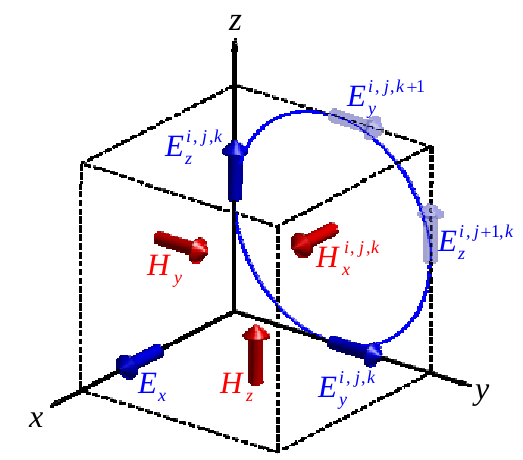
\includegraphics[width=0.5\textwidth]{YeeGridHx.png}
  \caption{Yee Grid Hx}
  \label{fig:YeeGridHx}
\end{figure}

\begin{align}
  \label{eq:YeeGridHx}
  \frac{\partial E_z}{\partial y} - \frac{\partial E_y}{\partial z} = -\frac{\mu_{xx}}{c_0}\frac{\partial\tilde{H}_x}{\partial t}
  \longrightarrow\\
  \frac{E_{z}^{i,j+1,k}\mid_{t} - E_{z}^{i,j,k}\mid_{t}}{\Delta y} - \frac{E_{y}^{i,j,k+1}\mid_{t} - E_{y}^{i,j,k}\mid_{t}}{\Delta z} = -\frac{\mu_{xx}^{i,j,k}}{c_0} \frac{\tilde{H}_{x}^{i,j,k}\mid_{t+\frac  {\Delta t}{2}} - \tilde{H}_{x}^{i,j,k}\mid_{t-\frac{\Delta t}{2}}}{\Delta t}\notag
\end{align}


Hy - Figure \ref{fig:YeeGridHy} Equation \eqref{eq:YeeGridHy} 

\begin{figure}[h]
  \centering
    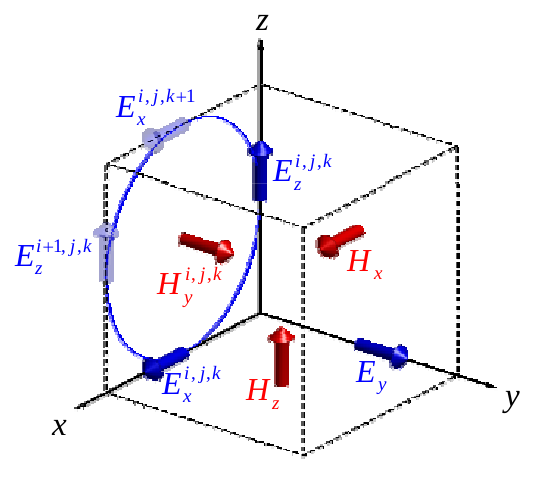
\includegraphics[width=0.5\textwidth]{YeeGridHy.png}
  \caption{Yee Grid Hy}
  \label{fig:YeeGridHy}
\end{figure}

\begin{align}
  \label{eq:YeeGridHy}
  \frac{\partial E_x}{\partial z} - \frac{\partial E_z}{\partial x} = -\frac{\mu_{yy}}{c_0}\frac{\partial\tilde{H}_y}{\partial t}
  \longrightarrow\\
  \frac{E_{x}^{i,j,k+1}\mid_{t} - E_{x}^{i,j,k}\mid_{t}}{\Delta z} - \frac{E_{z}^{i+1,j,k}\mid_{t} - E_{z}^{i,j,k}\mid_{t}}{\Delta x} = -\frac{\mu_{yy}^{i,j,k}}{c_0} \frac{\tilde{H}_{y}^{i,j,k}\mid_{t+\frac  {\Delta t}{2}} - \tilde{H}_{y}^{i,j,k}\mid_{t-\frac{\Delta t}{2}}}{\Delta t}\notag
\end{align}


Hz - Figure \ref{fig:YeeGridHz} Equation \eqref{eq:YeeGridHz} 

\begin{figure}[h]
  \centering
    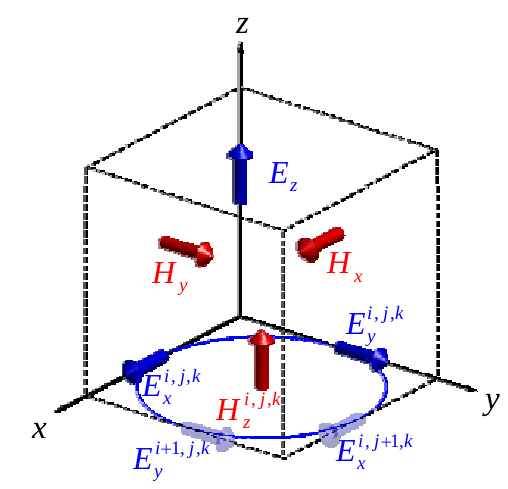
\includegraphics[width=0.5\textwidth]{YeeGridHz.png}
  \caption{Yee Grid Hz}
  \label{fig:YeeGridHz}
\end{figure}

\begin{align}
  \label{eq:YeeGridHz}
  \frac{\partial E_y}{\partial x} - \frac{\partial E_x}{\partial y} = -\frac{\mu_{zz}}{c_0}\frac{\partial\tilde{H}_z}{\partial t}
  \longrightarrow\\
  \frac{E_{y}^{i+1,j,k}\mid_{t} - E_{y}^{i,j,k}\mid_{t}}{\Delta x} - \frac{E_{x}^{i,j+1,k}\mid_{t} - E_{x}^{i,j,k}\mid_{t}}{\Delta y} = -\frac{\mu_{zz}^{i,j,k}}{c_0} \frac{\tilde{H}_{z}^{i,j,k}\mid_{t+\frac  {\Delta t}{2}} - \tilde{H}_{z}^{i,j,k}\mid_{t-\frac{\Delta t}{2}}}{\Delta t}\notag
\end{align}


Ex - Figure \ref{fig:YeeGridEx} Equation \eqref{eq:YeeGridEx} 

\begin{figure}[h]
  \centering
    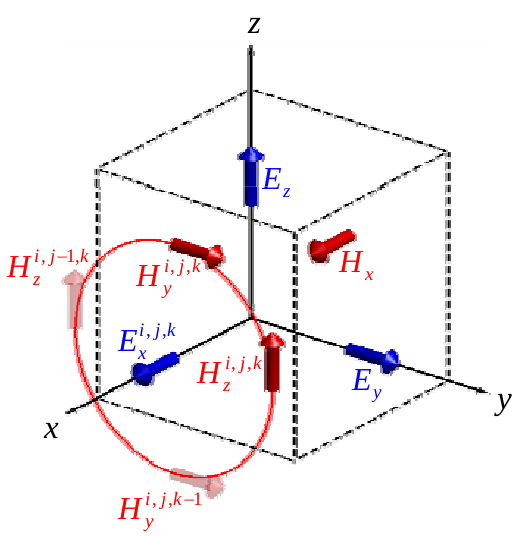
\includegraphics[width=0.5\textwidth]{YeeGridEx.png}
  \caption{Yee Grid Ex}
  \label{fig:YeeGridEx}
\end{figure}

\begin{align}
  \label{eq:YeeGridEx}
  \frac{\partial \tilde{H}_z}{\partial y} - \frac{\partial \tilde{H}_y}{\partial z} = -\frac{\epsilon_{xx}}{c_0}\frac{\partial E_x}{\partial t}
  \longrightarrow\\
  \frac{\tilde{H}_{z}^{i,j,k}\mid_{t+\frac{\Delta t}{2}} - \tilde{H}_{z}^{i,j-1,k}\mid_{t+\frac  {\Delta t}{2}}}{\Delta y} - \frac{\tilde{H}_{y}^{i,j,k}\mid_{t+\frac  {\Delta t}{2}} - \tilde{H}_{y}^{i,j,k-1}\mid_{t+\frac  {\Delta t}{2}}}{\Delta z} = \frac{\epsilon_{xx}^{i,j,k}}{c_0} \frac{E_{x}^{i,j,k}\mid_{t+\Delta t} - E_{x}^{i,j,k}\mid_{t}}{\Delta t}\notag
\end{align}


Ey - Figure \ref{fig:YeeGridEy} Equation \eqref{eq:YeeGridEy} 

\begin{figure}[h]
  \centering
    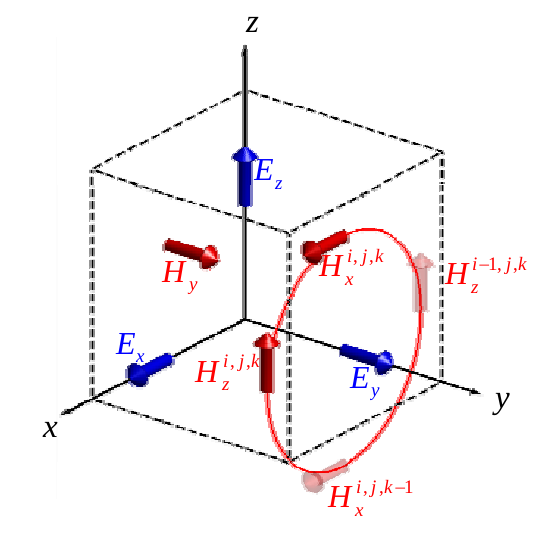
\includegraphics[width=0.5\textwidth]{YeeGridEy.png}
  \caption{Yee Grid Ey}
  \label{fig:YeeGridEy}
\end{figure}

\begin{align}
  \label{eq:YeeGridEy}
  \frac{\partial \tilde{H}_x}{\partial z} - \frac{\partial \tilde{H}_z}{\partial x} = -\frac{\epsilon_{yy}}{c_0}\frac{\partial E_y}{\partial t}
  \longrightarrow\\
  \frac{\tilde{H}_{x}^{i,j,k}\mid_{t+\frac{\Delta t}{2}} - \tilde{H}_{x}^{i,j,k-1}\mid_{t+\frac  {\Delta t}{2}}}{\Delta z} - \frac{\tilde{H}_{z}^{i,j,k}\mid_{t+\frac  {\Delta t}{2}} - \tilde{H}_{z}^{i-1,j,k}\mid_{t+\frac  {\Delta t}{2}}}{\Delta x} = \frac{\epsilon_{yy}^{i,j,k}}{c_0} \frac{E_{y}^{i,j,k}\mid_{t+\Delta t} - E_{y}^{i,j,k}\mid_{t}}{\Delta t}\notag
\end{align}


Ez - Figure \ref{fig:YeeGridEz} Equation \eqref{eq:YeeGridEz} 

\begin{figure}[h]
  \centering
    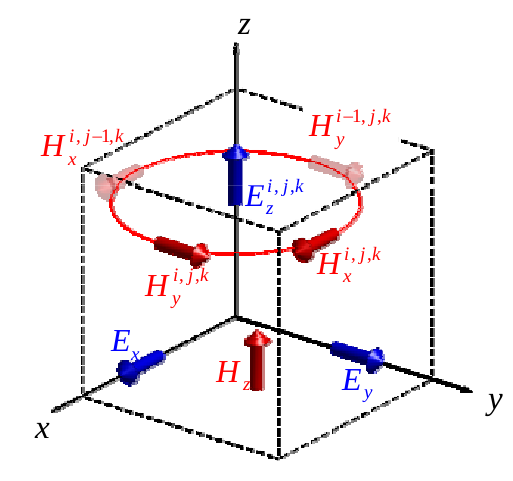
\includegraphics[width=0.5\textwidth]{YeeGridEz.png}
  \caption{Yee Grid Ez}
  \label{fig:YeeGridEz}
\end{figure}

\begin{align}
  \label{eq:YeeGridEz}
  \frac{\partial \tilde{H}_y}{\partial x} - \frac{\partial \tilde{H}_x}{\partial y} = -\frac{\epsilon_{zz}}{c_0}\frac{\partial E_z}{\partial t}
  \longrightarrow\\
  \frac{\tilde{H}_{y}^{i,j,k}\mid_{t+\frac{\Delta t}{2}} - \tilde{H}_{y}^{i-1,j,k}\mid_{t+\frac  {\Delta t}{2}}}{\Delta x} - \frac{\tilde{H}_{x}^{i,j,k}\mid_{t+\frac  {\Delta t}{2}} - \tilde{H}_{x}^{i,j-1,k}\mid_{t+\frac  {\Delta t}{2}}}{\Delta y} = \frac{\epsilon_{zz}^{i,j,k}}{c_0} \frac{E_{z}^{i,j,k}\mid_{t+\Delta t} - E_{z}^{i,j,k}\mid_{t}}{\Delta t}\notag
\end{align}


\textbf{Summary of Finite-Difference Equations}

The six sets equations below are our Finite-Difference equations derived from Maxwell's Equations.  These equations we will use to derive equations for 1D, 2D, and 3D update equations for our FDTD algorithms.

\begin{equation*}
  \frac{\partial E_z}{\partial y} - \frac{\partial E_y}{\partial z} = -\frac{\mu_{xx}}{c_0}\frac{\partial\tilde{H}_x}{\partial t}
\end{equation*}

\begin{equation*}
  \frac{\partial E_x}{\partial z} - \frac{\partial E_z}{\partial x} = -\frac{\mu_{yy}}{c_0}\frac{\partial\tilde{H}_y}{\partial t}
\end{equation*}

\begin{equation*}
  \frac{\partial E_y}{\partial x} - \frac{\partial E_x}{\partial y} = -\frac{\mu_{zz}}{c_0}\frac{\partial\tilde{H}_z}{\partial t}
\end{equation*}

\begin{equation*}
  \frac{\partial \tilde{H}_z}{\partial y} - \frac{\partial \tilde{H}_y}{\partial z} = -\frac{\epsilon_{xx}}{c_0}\frac{\partial E_x}{\partial t}
\end{equation*}

\begin{equation*}
  \frac{\partial \tilde{H}_x}{\partial z} - \frac{\partial \tilde{H}_z}{\partial x} = -\frac{\epsilon_{yy}}{c_0}\frac{\partial E_y}{\partial t}
\end{equation*}

\begin{equation*}
  \frac{\partial \tilde{H}_y}{\partial x} - \frac{\partial \tilde{H}_x}{\partial y} = -\frac{\epsilon_{zz}}{c_0}\frac{\partial E_z}{\partial t}
\end{equation*}

\[\longrightarrow\]

\begin{equation*}
  \frac{E_{z}^{i,j+1,k}\mid_{t} - E_{z}^{i,j,k}\mid_{t}}{\Delta y} - \frac{E_{y}^{i,j,k+1}\mid_{t} - E_{y}^{i,j,k}\mid_{t}}{\Delta z} = -\frac{\mu_{xx}^{i,j,k}}{c_0} \frac{\tilde{H}_{x}^{i,j,k}\mid_{t+\frac  {\Delta t}{2}} - \tilde{H}_{x}^{i,j,k}\mid_{t-\frac{\Delta t}{2}}}{\Delta t}\notag
\end{equation*}

\begin{equation*}
  \frac{E_{x}^{i,j,k+1}\mid_{t} - E_{x}^{i,j,k}\mid_{t}}{\Delta z} - \frac{E_{z}^{i+1,j,k}\mid_{t} - E_{z}^{i,j,k}\mid_{t}}{\Delta x} = -\frac{\mu_{yy}^{i,j,k}}{c_0} \frac{\tilde{H}_{y}^{i,j,k}\mid_{t+\frac  {\Delta t}{2}} - \tilde{H}_{y}^{i,j,k}\mid_{t-\frac{\Delta t}{2}}}{\Delta t}\notag
\end{equation*}

\begin{equation*}
  \frac{E_{y}^{i+1,j,k}\mid_{t} - E_{y}^{i,j,k}\mid_{t}}{\Delta x} - \frac{E_{x}^{i,j+1,k}\mid_{t} - E_{x}^{i,j,k}\mid_{t}}{\Delta y} = -\frac{\mu_{zz}^{i,j,k}}{c_0} \frac{\tilde{H}_{z}^{i,j,k}\mid_{t+\frac  {\Delta t}{2}} - \tilde{H}_{z}^{i,j,k}\mid_{t-\frac{\Delta t}{2}}}{\Delta t}\notag
\end{equation*}

\begin{equation*}
  \frac{\tilde{H}_{z}^{i,j,k}\mid_{t+\frac{\Delta t}{2}} - \tilde{H}_{z}^{i,j-1,k}\mid_{t+\frac  {\Delta t}{2}}}{\Delta y} - \frac{\tilde{H}_{y}^{i,j,k}\mid_{t+\frac  {\Delta t}{2}} - \tilde{H}_{y}^{i,j,k-1}\mid_{t+\frac  {\Delta t}{2}}}{\Delta z} = \frac{\epsilon_{xx}^{i,j,k}}{c_0} \frac{E_{x}^{i,j,k}\mid_{t+\Delta t} - E_{x}^{i,j,k}\mid_{t}}{\Delta t}\notag
\end{equation*}

\begin{equation*}
  \frac{\tilde{H}_{x}^{i,j,k}\mid_{t+\frac{\Delta t}{2}} - \tilde{H}_{x}^{i,j,k-1}\mid_{t+\frac  {\Delta t}{2}}}{\Delta z} - \frac{\tilde{H}_{z}^{i,j,k}\mid_{t+\frac  {\Delta t}{2}} - \tilde{H}_{z}^{i-1,j,k}\mid_{t+\frac  {\Delta t}{2}}}{\Delta x} = \frac{\epsilon_{yy}^{i,j,k}}{c_0} \frac{E_{y}^{i,j,k}\mid_{t+\Delta t} - E_{y}^{i,j,k}\mid_{t}}{\Delta t}\notag
\end{equation*}

\begin{equation*}
  \frac{\tilde{H}_{y}^{i,j,k}\mid_{t+\frac{\Delta t}{2}} - \tilde{H}_{y}^{i-1,j,k}\mid_{t+\frac  {\Delta t}{2}}}{\Delta x} - \frac{\tilde{H}_{x}^{i,j,k}\mid_{t+\frac  {\Delta t}{2}} - \tilde{H}_{x}^{i,j-1,k}\mid_{t+\frac  {\Delta t}{2}}}{\Delta y} = \frac{\epsilon_{zz}^{i,j,k}}{c_0} \frac{E_{z}^{i,j,k}\mid_{t+\Delta t} - E_{z}^{i,j,k}\mid_{t}}{\Delta t}\notag
\end{equation*}



\textbf{Reduce to One-Dimension}

We will reduce our Finite-Difference Equations to 1D.  This means that we will have material that is uniform in two directions.  
This uniform material will cause the fields to be uniform as well.  The change in material in our case we will define to be in the z-drection there for in the x anx y direction
will be uniform.  This means that the directives in this direction will also equal zero.

\begin{equation*}
 \frac{\partial}{\partial x} = \frac{\partial}{\partial y}=0
\end{equation*}

\begin{figure}[h]
  \centering
    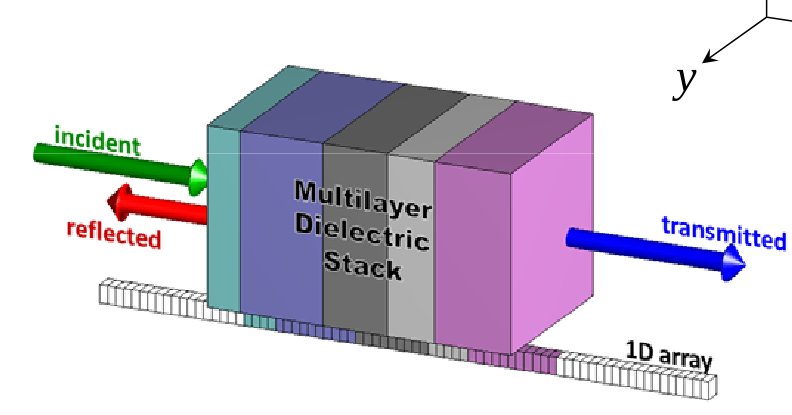
\includegraphics[width=0.5\textwidth]{Slabs1D.png}
  \caption{1D Problem}
\end{figure}


From our Finite-Difference equations we need to cancel out the x and y derivates that are zero.


\begin{equation*}
  \cancel{\frac{\partial E_z}{\partial y}} - \frac{\partial E_y}{\partial z} = -\frac{\mu_{xx}}{c_0}\frac{\partial\tilde{H}_x}{\partial t}
\end{equation*}

\begin{equation*}
  \frac{\partial E_x}{\partial z} - \cancel{\frac{\partial E_z}{\partial x}} = -\frac{\mu_{yy}}{c_0}\frac{\partial\tilde{H}_y}{\partial t}
\end{equation*}

\begin{equation*}
  \cancel{\frac{\partial E_y}{\partial x}} - \cancel{\frac{\partial E_x}{\partial y}} = -\frac{\mu_{zz}}{c_0}\frac{\partial\tilde{H}_z}{\partial t}
\end{equation*}

\begin{equation*}
  \cancel{\frac{\partial \tilde{H}_z}{\partial y}} - \frac{\partial \tilde{H}_y}{\partial z} = -\frac{\epsilon_{xx}}{c_0}\frac{\partial E_x}{\partial t}
\end{equation*}

\begin{equation*}
  \frac{\partial \tilde{H}_x}{\partial z} - \cancel{\frac{\partial \tilde{H}_z}{\partial x}} = -\frac{\epsilon_{yy}}{c_0}\frac{\partial E_y}{\partial t}
\end{equation*}

\begin{equation*}
  \cancel{\frac{\partial \tilde{H}_y}{\partial x}} - \cancel{\frac{\partial \tilde{H}_x}{\partial y}} = -\frac{\epsilon_{zz}}{c_0}\frac{\partial E_z}{\partial t}
\end{equation*}

\[\longrightarrow\]

\begin{equation*}
  \cancel{\frac{E_{z}^{i,j+1,k}\mid_{t} - E_{z}^{i,j,k}\mid_{t}}{\Delta y}} - \frac{E_{y}^{i,j,k+1}\mid_{t} - E_{y}^{i,j,k}\mid_{t}}{\Delta z} = -\frac{\mu_{xx}^{i,j,k}}{c_0} \frac{\tilde{H}_{x}^{i,j,k}\mid_{t+\frac  {\Delta t}{2}} - \tilde{H}_{x}^{i,j,k}\mid_{t-\frac{\Delta t}{2}}}{\Delta t}\notag
\end{equation*}

\begin{equation*}
  \frac{E_{x}^{i,j,k+1}\mid_{t} - E_{x}^{i,j,k}\mid_{t}}{\Delta z} - \cancel{\frac{E_{z}^{i+1,j,k}\mid_{t} - E_{z}^{i,j,k}\mid_{t}}{\Delta x}} = -\frac{\mu_{yy}^{i,j,k}}{c_0} \frac{\tilde{H}_{y}^{i,j,k}\mid_{t+\frac  {\Delta t}{2}} - \tilde{H}_{y}^{i,j,k}\mid_{t-\frac{\Delta t}{2}}}{\Delta t}\notag
\end{equation*}

\begin{equation*}
  \cancel{\frac{E_{y}^{i+1,j,k}\mid_{t} - E_{y}^{i,j,k}\mid_{t}}{\Delta x}} - \cancel{\frac{E_{x}^{i,j+1,k}\mid_{t} - E_{x}^{i,j,k}\mid_{t}}{\Delta y}} = -\frac{\mu_{zz}^{i,j,k}}{c_0} \frac{\tilde{H}_{z}^{i,j,k}\mid_{t+\frac  {\Delta t}{2}} - \tilde{H}_{z}^{i,j,k}\mid_{t-\frac{\Delta t}{2}}}{\Delta t}\notag
\end{equation*}

\begin{equation*}
  \cancel{\frac{\tilde{H}_{z}^{i,j,k}\mid_{t+\frac{\Delta t}{2}} - \tilde{H}_{z}^{i,j-1,k}\mid_{t+\frac  {\Delta t}{2}}}{\Delta y}} - \frac{\tilde{H}_{y}^{i,j,k}\mid_{t+\frac  {\Delta t}{2}} - \tilde{H}_{y}^{i,j,k-1}\mid_{t+\frac  {\Delta t}{2}}}{\Delta z} = \frac{\epsilon_{xx}^{i,j,k}}{c_0} \frac{E_{x}^{i,j,k}\mid_{t+\Delta t} - E_{x}^{i,j,k}\mid_{t}}{\Delta t}\notag
\end{equation*}

\begin{equation*}
  \frac{\tilde{H}_{x}^{i,j,k}\mid_{t+\frac{\Delta t}{2}} - \tilde{H}_{x}^{i,j,k-1}\mid_{t+\frac  {\Delta t}{2}}}{\Delta z} - \cancel{\frac{\tilde{H}_{z}^{i,j,k}\mid_{t+\frac  {\Delta t}{2}} - \tilde{H}_{z}^{i-1,j,k}\mid_{t+\frac  {\Delta t}{2}}}{\Delta x}} = \frac{\epsilon_{yy}^{i,j,k}}{c_0} \frac{E_{y}^{i,j,k}\mid_{t+\Delta t} - E_{y}^{i,j,k}\mid_{t}}{\Delta t}\notag
\end{equation*}

\begin{equation*}
  \cancel{\frac{\tilde{H}_{y}^{i,j,k}\mid_{t+\frac{\Delta t}{2}} - \tilde{H}_{y}^{i-1,j,k}\mid_{t+\frac  {\Delta t}{2}}}{\Delta x}} - \cancel{\frac{\tilde{H}_{x}^{i,j,k}\mid_{t+\frac  {\Delta t}{2}} - \tilde{H}_{x}^{i,j-1,k}\mid_{t+\frac  {\Delta t}{2}}}{\Delta y}} = \frac{\epsilon_{zz}^{i,j,k}}{c_0} \frac{E_{z}^{i,j,k}\mid_{t+\Delta t} - E_{z}^{i,j,k}\mid_{t}}{\Delta t}\notag
\end{equation*}




















\end{document}

